\documentclass{article}
\usepackage{amsmath}
\usepackage{amsfonts, amsthm, amssymb}
\usepackage{graphicx}
\usepackage[colorlinks]{hyperref}
\usepackage[parfill]{parskip}
\usepackage{algpseudocode}
\usepackage{algorithm}
\usepackage{enumerate}
\usepackage[shortlabels]{enumitem}
\usepackage{fullpage}
\usepackage{mathtools}
\usepackage{subcaption}
\usepackage{tikz}

\usepackage{natbib}
\renewcommand{\bibname}{REFERENCES}
\renewcommand{\bibsection}{\subsubsection*{\bibname}}

\DeclareFontFamily{U}{mathx}{\hyphenchar\font45}
\DeclareFontShape{U}{mathx}{m}{n}{<-> mathx10}{}
\DeclareSymbolFont{mathx}{U}{mathx}{m}{n}
\DeclareMathAccent{\wb}{0}{mathx}{"73}

\DeclarePairedDelimiterX{\norm}[1]{\lVert}{\rVert}{#1}

\newcommand{\eqdist}{\ensuremath{\stackrel{d}{=}}}
\newcommand{\Graph}{\mathcal{G}}
\newcommand{\Reals}{\mathbb{R}}
\newcommand{\Identity}{\mathbb{I}}
\newcommand{\Xsetistiid}{\overset{\text{i.i.d}}{\sim}}
\newcommand{\convprob}{\overset{p}{\to}}
\newcommand{\convdist}{\overset{w}{\to}}
\newcommand{\Expect}[1]{\mathbb{E}\left[ #1 \right]}
\newcommand{\Risk}[2][P]{\mathcal{R}_{#1}\left[ #2 \right]}
\newcommand{\Prob}[1]{\mathbb{P}\left( #1 \right)}
\newcommand{\iset}{\mathbf{i}}
\newcommand{\jset}{\mathbf{j}}
\newcommand{\myexp}[1]{\exp \{ #1 \}}
\newcommand{\abs}[1]{\left \lvert #1 \right \rvert}
\newcommand{\restr}[2]{\ensuremath{\left.#1\right|_{#2}}}
\newcommand{\ext}[1]{\widetilde{#1}}
\newcommand{\set}[1]{\left\{#1\right\}}
\newcommand{\seq}[1]{\set{#1}_{n \in \N}}
\newcommand{\Xsetotp}[2]{\langle #1, #2 \rangle}
\newcommand{\floor}[1]{\left\lfloor #1 \right\rfloor}
\newcommand{\Var}{\mathrm{Var}}
\newcommand{\Cov}{\mathrm{Cov}}
\newcommand{\Xsetiam}{\mathrm{diam}}

\newcommand{\emC}{C_n}
\newcommand{\emCpr}{C'_n}
\newcommand{\emCthick}{C^{\sigma}_n}
\newcommand{\emCprthick}{C'^{\sigma}_n}
\newcommand{\emS}{S^{\sigma}_n}
\newcommand{\estC}{\widehat{C}_n}
\newcommand{\hC}{\hat{C^{\sigma}_n}}
\newcommand{\vol}{\text{vol}}
\newcommand{\spansp}{\mathrm{span}~}
\newcommand{\1}{\mathbf{1}}

\newcommand{\Linv}{L^{\Xsetagger}}
\DeclareMathOperator*{\argmin}{argmin}
\DeclareMathOperator*{\argmax}{argmax}

\newcommand{\emF}{\mathbb{F}_n}
\newcommand{\emG}{\mathbb{G}_n}
\newcommand{\emP}{\mathbb{P}_n}
\newcommand{\F}{\mathcal{F}}
\newcommand{\D}{\mathcal{D}}
\newcommand{\R}{\mathcal{R}}
\newcommand{\Rd}{\Reals^d}
\newcommand{\Nbb}{\mathbb{N}}

%%% Vectors
\newcommand{\thetast}{\theta^{\star}}
\newcommand{\betap}{\beta^{(p)}}
\newcommand{\betaq}{\beta^{(q)}}
\newcommand{\vardeltapq}{\varDelta^{(p,q)}}


%%% Matrices
\newcommand{\X}{X} % no bold
\newcommand{\Y}{Y} % no bold
\newcommand{\Z}{Z} % no bold
\newcommand{\Lgrid}{L_{\grid}}
\newcommand{\Xsetgrid}{D_{\grid}}
\newcommand{\Linvgrid}{L_{\grid}^{\Xsetagger}}
\newcommand{\Lap}{{\bf L}}
\newcommand{\NLap}{{\bf N}}
\newcommand{\PLap}{{\bf P}}

%%% Sets and classes
\newcommand{\Xset}{\mathcal{X}}
\newcommand{\Sset}{\mathcal{S}}
\newcommand{\Hclass}{\mathcal{H}}
\newcommand{\Pclass}{\mathcal{P}}
\newcommand{\Leb}{L}
\newcommand{\mc}[1]{\mathcal{#1}}

%%% Distributions and related quantities
\newcommand{\Pbb}{\mathbb{P}}
\newcommand{\Ebb}{\mathbb{E}}
\newcommand{\Qbb}{\mathbb{Q}}
\newcommand{\Ibb}{\mathbb{I}}

%%% Operators
\newcommand{\Tadj}{T^{\star}}
\newcommand{\Xsetive}{\mathrm{div}}
\newcommand{\Xsetif}{\mathop{}\!\mathrm{d}}
\newcommand{\gradient}{\mathcal{D}}
\newcommand{\Hessian}{\mathcal{D}^2}
\newcommand{\dotp}[2]{\langle #1, #2 \rangle}
\newcommand{\Dotp}[2]{\Bigl\langle #1, #2 \Bigr\rangle}

%%% Misc
\newcommand{\grid}{\mathrm{grid}}
\newcommand{\critr}{R_n}
\newcommand{\Xsetx}{\,dx}
\newcommand{\Xsety}{\,dy}
\newcommand{\Xsetr}{\,dr}
\newcommand{\Xsetxpr}{\,dx'}
\newcommand{\Xsetypr}{\,dy'}
\newcommand{\wt}[1]{\widetilde{#1}}
\newcommand{\wh}[1]{\widehat{#1}}
\newcommand{\ol}[1]{\overline{#1}}
\newcommand{\spec}{\mathrm{spec}}
\newcommand{\LE}{\mathrm{LE}}
\newcommand{\LS}{\mathrm{LS}}
\newcommand{\OS}{\mathrm{OS}}
\newcommand{\PLS}{\mathrm{PLS}}

%%% Order of magnitude
\newcommand{\soom}{\sim}

% \newcommand{\span}{\textrm{span}}

\newtheoremstyle{alden}
{6pt} % Space above
{6pt} % Space below
{} % Body font
{} % Indent amount
{\bfseries} % Theorem head font
{.} % Punctuation after theorem head
{.5em} % Space after theorem head
{} % Theorem head spec (can be left empty, meaning `normal')

\theoremstyle{alden} 


\newtheoremstyle{aldenthm}
{6pt} % Space above
{6pt} % Space below
{\itshape} % Body font
{} % Indent amount
{\bfseries} % Theorem head font
{.} % Punctuation after theorem head
{.5em} % Space after theorem head
{} % Theorem head spec (can be left empty, meaning `normal')

\theoremstyle{aldenthm}
\newtheorem{theorem}{Theorem}
\newtheorem{conjecture}{Conjecture}
\newtheorem{lemma}{Lemma}
\newtheorem{example}{Example}
\newtheorem{corollary}{Corollary}
\newtheorem{proposition}{Proposition}
\newtheorem{assumption}{Assumption}
\newtheorem{remark}{Remark}


\theoremstyle{definition}
\newtheorem{definition}{Definition}[section]

\theoremstyle{remark}

\begin{document}
\title{Notes on: Revision for JMLR Submission on Local Spectral Clustering of Density Upper Level Sets}
\author{Alden Green}
\date{\today}
\maketitle

Recall: our Theorem 5 (JMLR numbering) says that with high probability, the following statement holds: when the PPR algorithm is properly initialized, the resulting estimator $\wh{C}$ of an empirical density cluster $\mc{C}_{\sigma}[X]$ satisfies
\begin{equation}
\label{eqn:volume_ssd_ppr}
\frac{\Delta(\wh{C},C_{\sigma}[X])}{\vol_{n,r}(\mc{C}_{\sigma}[X])} \leq c \cdot \kappa(\mc{C}).
\end{equation}
Both reviewers and the editor treated Theorem~5 as our main result, and viewed it as too weak, in related but slightly different ways. Specifically, they worried that:
\begin{itemize}
	\item \textbf{Reviewer 1.} For an example provided in our experiments section, the right hand side is (many times) larger than $1$. Since the trivial estimator $\wh{C} = \emptyset$ will always have
	\begin{equation*}
	\frac{\Delta(\emptyset,C_{\sigma}[X])}{\vol_{n,r}(\mc{C}_{\sigma}[X])}  = 1,
	\end{equation*}
	our bound is vacuous.
	\item \textbf{Reviewer 2.} The right hand side of~\eqref{eqn:volume_ssd_ppr} does not go to $0$ as $n \to \infty$. 
	\item \textbf{Editor.} ``...either the three of us did not get the 
	point of Theorem 5, in which case the presentation
	is obviously not satisfying, or Theorem 5 is not
	as strong as one would like to have it."
\end{itemize}

Both Reviewer 1 and Reviewer 2 make accurate statements, motivating the following pair of research questions:
\begin{enumerate}
	\item \textbf{Addressing the concerns of Reviewer 1.} What are some distributions $P$ and resulting density clusters $\mc{C}$ for which our bound is not vacuous, i.e. for which
	\begin{equation*}
	c \cdot \kappa(\mc{C}) < 1?
	\end{equation*}
	\item \textbf{Addressing the concerns of Reviewer 2.} Should we expect the right hand side of~\eqref{eqn:volume_ssd_ppr} to go to $0$ as $n \to \infty$?
\end{enumerate}
We address these concerns in the following two sections.

\section{Concerns of Reviewer 1}

\subsection{Uniform rectangles + $\epsilon$-background noise model.}
Let us recall the model used in the construction of our ``hard case''. Letting $\theta = (\epsilon,w,h)$, the distribution $P = P_{\theta}$ is a mixtures of uniforms over the unit square $[-1,1]^2$:
\begin{equation*}
P_{\theta} := \frac{1 - \epsilon}{2} P_{(1)} + \frac{1 - \epsilon}{2} P_{(2)} + \epsilon Q;
\end{equation*}
here $Q$ is the uniform distribution over $[-1,1]^2$, and the mixture component $P_{(i)}$ is the uniform distribution over the rectangle $\mc{C}_{(i)}$, 
\begin{equation*}
\mc{C}_{(i)} := c_{(i)} + \frac{1}{2}\Bigl([-w,w] \times [-h,h]\Bigr)
\end{equation*}
with $c_{(1)} = (-.5,0)$ and $c_{(2)} = (.5,0)$, and. Letting $f_{\theta}$ be the density function of $P_{\theta}$---which has the simple closed form expression
\begin{equation*}
f_{\theta}(x) =
\begin{cases}
\frac{(1 - \epsilon)}{2wh} + \frac{1}{4}\epsilon,& ~~ x \in \mc{C}_{(i)} \\
\frac{1}{4}\epsilon,& ~~ x \in [-1,1]^2 \setminus \bigl(\mc{C}_{(1)} \cup \mc{C}_{(2)}\bigr)
\end{cases}
\end{equation*}
---it is clear that $\mc{C}_{(1)}$ and $\mc{C}_{(2)}$ have higher density than the rest of $[-1,1]^2$, and in particular that for any $\epsilon/4 < \lambda \leq (1 - \epsilon)/(2wh) + \epsilon/4$ we have $\mathbb{C}_f(\lambda) = \{\mc{C}_{(1)}, \mc{C}_{(2)}\}$. 

\paragraph{Our bound.}
To be more explicit, our bound upper bound on the volume of the symmetric set difference is given by
\begin{equation}
\label{eqn:volume_ssd_ppr_explicit}
\frac{\Delta(\wh{C},\mc{C}_{\sigma}[X])}{\vol_{n,r}(\mc{C}_{\sigma}[X])} \leq 2180 \cdot \Phi_u(\mc{C}) \cdot \tau_{u}(\mc{C}),
\end{equation}
i.e. the constant in~\eqref{eqn:volume_ssd_ppr} is $c = 2180$, and the condition number $\kappa(\mc{C})$ is equal to the product of (upper bounds on) the normalized cut $\Phi_u(\mc{C})$ and mixing time $\tau_u(\mc{C})$. Technically speaking the density clusters $\mc{C}_{(i)}$ do not satisfy our assumptions on density clusters $\mc{C}_{\sigma}$, but modulo some additional bookkeeping we can compute the following upper bounds:
\begin{equation*}
\Phi_u(\mc{C}) = 
\end{equation*}


\paragraph{}

\begin{itemize}
	\item There exist choices of $\theta$ for which:
	\begin{enumerate}[(i)]
		\item  Our bound on 
		\begin{equation*}
		\frac{\Delta(\wh{C},\mc{C}[X])}{\vol_{n,r}(\mc{C}[X])}
		\end{equation*}
		will be less than $1$. 
		\item 
		\begin{equation*}
		\frac{\Delta(\wh{C},\mc{C}[X])}{\vol_{n,r}(\mc{C}[X])} < 1,
		\end{equation*}
		but any bound based on the results of \textcolor{red}{(Allen-Zhu)} will be $ > 1$.
	\end{enumerate}
	The point (i) is an obvious response to Reviewer 1. The concern is that the values of $\theta$ for which (i) holds are implausible, for instance if $\epsilon$ must be absurdly small. Point (ii) addresses this concern, giving the values of $\theta$ one should expect to derive for if one must use the results of \textcolor{red}{(Allen-Zhu)}. 
	\item \textbf{Rates of convergence in $\epsilon$.} As $\epsilon \to 0$, it is obvious that PPR will come to consistently recover $\mc{C}$. Our upper bound correctly reflects this fact. The following question is perhaps more interesting: does our upper bound correctly capture the rate of convergence?
\end{itemize}

\subsection{Other models?}

\textcolor{red}{(Discuss with Siva.)}


\section{Concerns of Reviewer 2}
We first point out that to the best of our knowledge, all other works on spectral clustering on random geometric graphs fall into three categories. 
\begin{enumerate}[(1)]
	\item Define clusters with respect to geometric conditions, obtain upper bound on classification error that does not go to $0$ as $n \to \infty$.
	\item Obtain consistency, but for clusters defined with respect to a continuum PDE or eigenfunction problem.
	\item Obtain consistency for geometrically defined clusters, by changing the algorithm.
\end{enumerate} 
Our work falls into category (1), and so trades a weaker result---non-vanishing upper bound on classification error---for a more natural definition of cluster. 

Of course, simply because other works in category (1) share the non-vanishing upper bound property does not mean that such a property is fundamental to the problem. We investigate the question empirically.

\subsection{Uniform rectangles + $\epsilon$-background noise model}

Let $X_1,\ldots,X_n$ be drawn from $P_{\theta}$, with $w = .5, h = 1$ and $\epsilon \approx .72$. In Figure~\ref{fig:fig1}, we plot the error---volume of the symmetric set difference, normalized by the volume of $\mc{C}_{(1)}$--- of PPR clustering against the sample size $n$. We see that PPR--even when optimally seeded, tuned, and with the optimal sweep cut taken---fails to consistently recover $\mc{C}_{(1)}$. 
\begin{figure}
	\centering
	\begin{subfigure}{.5\textwidth}
	\centering
	\includegraphics[width=.8\linewidth]{figures/11_05_2020/error.pdf}
	\end{subfigure}%
	\begin{subfigure}{.5\textwidth}
		\centering
		\includegraphics[width=.8\linewidth]{figures/11_05_2020/error_upper_bound.pdf}
	\end{subfigure}
	\caption{Error---$\Delta(\wh{C},\mc{C}[X])$ divided by $\vol_{n,r}(\mc{C}_{(1)}[X])$---of PPR clusters $\wh{C}$, averaged over 5 iterations. Different curves correspond to different values of radius $r$. For each value of radius $r$, a range of teleportation parameters $\alpha$ and sweep cuts was considered; we have plotted the smallest error among these ranges.}
	\label{fig:fig1}
\end{figure}

In Figures 2 and 3, we see what the set is that PPR actually recovers. The lesson is unsurprising: PPR trades off geometry for density, preferring an estimate $\wh{C}$ which is somewhat more geometrically well-behaved (i.e lower aspect ratio) even at the expense of including some low-density areas.
\begin{figure}
	\centering
	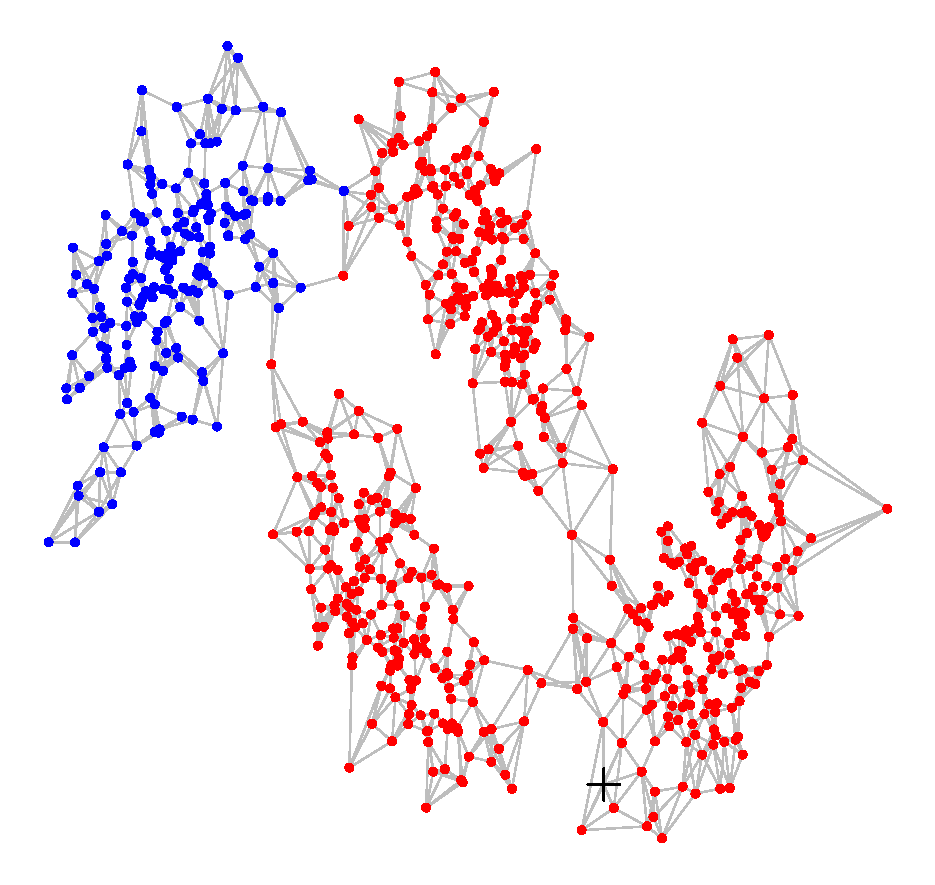
\includegraphics[width = .5\textwidth]{figures/11_05_2020/ppr_cluster.pdf}
	\caption{PPR cluster estimate, for different values of $r$.}
	\label{fig:fig2}
\end{figure}




\end{document}